\section{Multilinear Kakeya}
By the discussion in the introduction, functions with Fourier support in boxes near a parabola (left picture) are morally constant on polar boxes (right picture).
We will call boxes ``polar'' if they have the same orientation and the product of lengths of corresponding sides is $1$ (this is morally a special case of ``polar sets'' in convex analysis).
\begin{center}
\begin{tikzpicture}
\draw (-1,1) to[parabola through={(0,0)}] (1,1);
\begin{scope}[black,cm={0.3,0,0,0.09,(0,0)}]
\draw (-1,0) rectangle (1,1);
\end{scope}
\begin{scope}[black,cm={0.3,0.6,0,0.09,(1,1)}]
\draw (-1,0) rectangle (0,1);
\end{scope}
\end{tikzpicture}
\hspace{2cm}
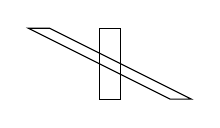
\begin{tikzpicture}[scale=3]
\begin{scope}[black,cm={0.09,0,0,0.3,(0,0)}]
\draw (0,0) rectangle (1,1);
\end{scope}
\begin{scope}[black,cm={0.09,0,-0.6,0.3,(0.3,0)}]
\draw (0,0) rectangle (1,1);
\end{scope}
\end{tikzpicture}
\end{center}
Let us provisionally call two arcs of the parabola \emph{transverse} if they are separated by more than their combined length.
As one sees in the picture, in dimension $2$ the interaction between two functions with transverse Fourier supports is relatively simple since they are basically constant in two different directions.
In particular, $L^{p}$ norms of their products can be morally computed by Fubini's theorem in terms of $L^{p}$ norms of the individual functions.
This is a big improvement over H\"older's inequality that needs $L^{2p}$ norms of the individual functions.
In this section we will see how transversality works in higher dimensions.

\begin{theorem}[Loomis--Whitney]\label{thm:Loomis-Whitney}
Let $n\geq 2$ and denote by $\pi_j: \R^n \rightarrow \R^{n-1}$ the linear map that forgets the $j^{th}$ coordinate:
\[
\pi_j( x_1, \dotsc, x_n) := (x_1, \dotsc, x_{j-1}, x_{j+1}, \dotsc, x_n).
\]
Suppose that $f_j: \R^{n-1} \to [0,\infty]$ are (measurable) functions.
Then the following integral inequality holds.
\begin{equation}\label{eq:Loomis-Whitney}
\int_{\R^n} \prod_{j=1}^n f_j \left( \pi_j(x) \right)^{\frac{1}{n-1}} \dif x
\le
\prod_{j=1}^n \norm{ f_j }_{L^1(\R^{n-1})}^{\frac{1}{n-1}}.
\end{equation}
\end{theorem}
\begin{proof}
By induction on $n$.
For $n=2$ the claim \eqref{eq:Loomis-Whitney} is a direct consequence of Fubini's theorem.
Suppose that the claim \eqref{eq:Loomis-Whitney} is known for some $n\geq 2$, we will now show it with $n$ replaced by $n+1$.
By H\"older's inequality, the inductive hypothesis, and again H\"older's inequality we obtain
\begin{align*}
\MoveEqLeft
\int_{\R^{n+1}} \prod_{j=1}^{n+1} f_j \left( \pi_j(x) \right)^{\frac{1}{n}} \dif x\\
&=
\int_{\R} \int_{\R^{n}} \prod_{j=1}^{n} f_j \left( \pi_j(x',x_{n+1}) \right)^{\frac{1}{n}} \cdot f_{n+1}(x')^{\frac{1}{n}} \dif x' \dif x_{n+1}\\
&\leq
\norm{f_{n+1}}_{1}^{1/n} \int_{\R} \Bigl( \int_{\R^{n}} \bigl( \prod_{j=1}^{n} f_j \left( \pi_j(x',x_{n+1}) \right)^{\frac{1}{n}} \bigr)^{n/(n-1)} \dif x' \Bigr)^{(n-1)/n} \dif x_{n+1}\\
&\leq
\norm{f_{n+1}}_{1}^{1/n} \int_{\R} \Bigl( \prod_{j=1}^{n} \norm{ f_j(\cdot,x_{n+1}) }_{L^{1}(\R^{n-1})}^{1/(n-1)} \Bigr)^{(n-1)/n} \dif x_{n+1}\\
&\leq
\norm{f_{n+1}}_{1}^{1/n} \prod_{j=1}^{n} \Bigl(\int_{\R} \norm{ f_j(\cdot,x_{n+1}) }_{L^{1}(\R^{n-1})} \dif x_{n+1} \Bigr)^{1/n}\\
&=
\norm{f_{n+1}}_{1}^{1/n} \prod_{j=1}^{n} \norm{ f_j }_{L^{1}(\R^{n})}^{1/n}
\end{align*}
as claimed.
\end{proof}

We will also use a variant in which the functions are constant in not necessarily othogonal directions.
\begin{corollary}[Affine invariant Loomis--Whitney]\label{cor:aff-inv-Loomis-Whitney}
Let $N_{1},\dotsc,N_{n} \in \R^{n}$ be unit vectors and $f_{j} : N_{j}^{\perp} \to [0,\infty]$ be measurable functions.
Then
\begin{equation}\label{eq:aff-inv-Loomis-Whitney}
\int_{\R^n} \prod_{j=1}^n (f_j \circ \pi_j)^{\frac{1}{n-1}}
\le
\abs[\big]{ N_{1} \wedge \dotsb \wedge N_{n} }^{-\frac{1}{n-1}}
\prod_{j=1}^n \norm{ f_j }_{L^1(N_{j}^{\perp})}^{\frac{1}{n-1}},
\end{equation}
where $\pi_{j}$ denotes the orthogonal projection onto $N_{j}^{\perp}$.
\end{corollary}
We recall that for column vectors $N_{1},\dotsc,N_{n} \in \R^{n}$ we have
\[
\abs[\big]{ N_{1} \wedge \dotsb \wedge N_{n} }
=
\abs*{ \det ( N_{1} \dots N_{n} )}.
\]
We will not be using any other properties of wedge products, so this indentity can be seen as an abbreviation.
\begin{proof}
Let $A$ be the linear map such that $A(e_{j})=N_{j}$, where $e_{1},\dotsc,e_{n}$ is the standard basis of $\R^{n}$.
By a change of variables and Theorem~\ref{thm:Loomis-Whitney} we have
\[
\int_{\R^n} \prod_{j=1}^n (f_j \circ \pi_j)^{\frac{1}{n-1}}
=
\abs{\det A} \int_{\R^n} \prod_{j=1}^n (f_j \circ \pi_j \circ A)^{\frac{1}{n-1}}
\leq
\abs{\det A} \prod_{j=1}^n \norm{f_j \circ \pi_j \circ A}_{L^{1}(e_{j}^{\perp})}^{\frac{1}{n-1}}.
\]
It remains to observe that $\pi_{j} \circ A$, viewed as a map $e_{j}^{\perp} \to N_{j}^{\perp}$, also has determinant $\det A$, so the above equals
\[
=
\abs{\det A} \prod_{j=1}^n \bigl( \abs{\det A}^{-1} \norm{f_j}_{L^{1}(N_{j}^{\perp})} \bigr)^{\frac{1}{n-1}}
=
\abs{\det A}^{-\frac{1}{n-1}} \prod_{j=1}^n \norm{f_j}_{L^{1}(N_{j}^{\perp})}^{\frac{1}{n-1}}.
\qedhere
\]
\end{proof}

The multilinear Kakeya inequality \cite{MR2275834} is a version of Loomis--Whitney in which instead of $n$ single directions we have $n$ families of directions.
The argument presented below (from \cite{MR3300318}) incurs a loss in the passage to a family of directions, and this loss restricts the kind of functions we can consider.
Instead of arbitrary functions $f \circ \pi$ we will use functions that are morally constant at some given scale $r$, and estimate the integral at a larger scale $R$.

An \emph{$r$-tube} is an infinite cylinder of radius $r$, or more precisely the $r$-neighborhood of its \emph{central line}, an affine subspace of dimension $1$.
The \emph{direction} of a tube is a unit vector parallel to its central line (there are two such vectors, the choice is not important).

\begin{theorem}[Multilinear Kakeya]\label{thm:mult-Kakeya}
For every $n\in\N$ and $\epsilon>0$ there exist $C_{1},C_{2}<\infty$ such that the following holds.
Let $0<\nu<1$ and $S_j \subset \mathbb{S}^{n-1}$ be such that for any vectors $v_j \in S_j$,
\[
\abs{ v_1 \wedge \dotsb \wedge v_n } \ge \nu.
\]
Let $r>0$ and for each $j=1,\dotsc,n$ let $\Tubes_{j}$ be a collection of tubes of radius $r$ in $\R^n$ whose directions lie in $S_j$.
Then for any ball $B$ of radius $R \geq r$ and any positive numbers $w_{T}$ we have
\begin{equation}\label{eq:mult-Kakeya}
\int_{B} \prod_{j=1}^n \Bigl( \sum_{T \in \Tubes_{j}} w_{T} \one_{T} \Bigr)^{\frac{1}{n-1}}
\le
C_{1} \nu^{-C_{2}} (R/r)^\epsilon r^{n} \prod_{j=1}^n \Bigl( \sum_{T \in \Tubes_{j}} w_{T} \Bigr)^{\frac{1}{n-1}}
\end{equation}
\end{theorem}

The power of $\nu$ in \eqref{eq:mult-Kakeya} can be taken the same as in the Loomis--Whitney inequality, and the loss $(R/r)^{\epsilon}$ can be removed.
However, this requires a completely different proof \cite{MR2746348} (see also \cite{arxiv:1807.09604} for a more general result).

\begin{proof}
By monotone convergence we may assume that the collections $\Tubes_{j}$ are finite.
By continuity we may assume that all coefficients $w_{T}$ are rational.
By scaling we may assume that they are all integers.
Allowing repetition of tubes in $\Tubes_{j}$ we may assume $w_{T}=1$ for all $T$.

Let $\delta \sim \nu^{C_{3}}$ be a dyadic number with $C_{3} = C_{3}(n,\epsilon)$ to be chosen later.
Replacing $\nu$ by $\nu/2$, say, and partitioning each $S_{j}$ into $O(\delta^{n-1})$ subsets of diameter $\ll \delta$ we may assume that each $S_{j}$ is a ball or radius $\ll \delta$ centered at some $\tilde{e}_{j} \in S^{n-1}$.
This loses a factor $\nu^{-C}$ in \eqref{eq:mult-Kakeya}.

With these reductions, for dyadic numbers $r\leq R$ let $\MK(R,r)$ be the smallest constant such that the inequality
\[
\int_{Q} \prod_{j=1}^n \Bigl( \sum_{T \in \Tubes_{j}} \one_{T} \Bigr)^{\frac{1}{n-1}}
\leq
\MK(R,r) \prod_{j=1}^n \abs{\Tubes_{j}}^{\frac{1}{n-1}}
\]
holds for any collections $\Tubes_{j}$ of tubes of radius $r$ and any cube $Q_{R}$ of side length $R$.
By scaling $\MK(R,r) = r^{n} \MK(R/r,1)$.
Estimating $\sum_{T \in \Tubes_{j}} \one_{T} \leq \abs{\Tubes_{j}}$ it becomes clear that $\MK(R,1) \lesssim R^{n}$.
It suffices to show that in fact $\MK(R,1) \lesssim R^{\epsilon}$.
We will obtain this estimate by going from scale $R$ to scale $1$ in many steps and using the Loomis--Whitney inequality at each step.

Let $\Tubes_{j}$ be collections of $1$-tubes with directions $\delta$-close to $\tilde{e}_{j}$.
We partition $Q_R$ into cubes $Q$ of side length $\sim \delta^{-1}$.
For each such cube $Q$ let $\Tubes_{j}(Q)$ be the set of tubes in $\Tubes_{j}$ that intersect $Q$.
For each $T \in \Tubes_{j}(Q)$, the intersection $T \cap Q$ is contained in a slightly thicker $2$-tube $T^{Q}$ with direction $\tilde{e}_{j}$.
Therefore,
\[
\int_{Q} \prod_{j=1}^n \Bigl( \sum_{T \in \Tubes_{j}} \one_{T} \Bigr)^{\frac{1}{n-1}}
=
\int_{Q} \prod_{j=1}^n \Bigl( \sum_{T \in \Tubes_{j}(Q)} \one_{T} \Bigr)^{\frac{1}{n-1}}
\leq
\int_{Q} \prod_{j=1}^n \Bigl( \sum_{T \in \Tubes_{j}} \one_{T^{Q}} \Bigr)^{\frac{1}{n-1}}.
\]
This last integral involves only $\tilde{e}_{j}$-parallel tubes of radius $2$, and by the Loomis--Whitney inequality it is
\[
\le
\nu^{-1/(n-1)} C_n \prod_{j=1}^n \abs{\Tubes_j(Q)}^{\frac{1}{n-1}}.
\]
\begin{center}
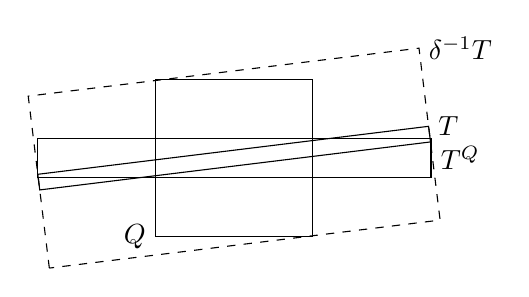
\begin{tikzpicture}
\draw (-1,-1) rectangle (1,1);
\draw (-1,-1) node[left] {$Q$};
\draw (-2.5,-0.25) rectangle (2.5,0.25) (2.5,0) node[right] {$T^{Q}$};
\draw[rotate=7] (-2.5,-0.1) rectangle (2.5,0.1) node[right] {$T$};
\draw[rotate=7,dashed] (-2.5,-1.1) rectangle (2.5,1.1) node[right] {$\delta^{-1} T$};
\end{tikzpicture}
\end{center}
For each $T \in \Tubes_{j}(Q)$ we have $\delta^{-1} T \supset Q$, where $\delta^{-1} T$ is the $\delta^{-1}$-tube with the same central line as $T$.
Therefore,
\[
\prod_{j=1}^n \abs{\Tubes_j(Q)}^{\frac{1}{n-1}}
\le
C_n \abs{Q}^{-1} \int_Q \prod_{j=1}^n \Bigl( \sum_{T \in \Tubes_{j}} \one_{\delta^{-1}T} \Bigr)^{\frac{1}{n-1}}.
\]
Summing over the cubes $Q$ we get
\[
\int_{Q_{R}} \prod_{j=1}^n \Bigl( \sum_{T \in \Tubes_{j}} \one_{T} \Bigr)^{\frac{1}{n-1}}
\leq
\nu^{-1/(n-1)} C_{n} \delta^{n} \int_{Q_{R}} \prod_{j=1}^n \Bigl( \sum_{T \in \Tubes_{j}} \one_{\delta^{-1}T} \Bigr)^{\frac{1}{n-1}}.
\]
By definition of $\MK$ the right-hand side is bounded by
\[
\nu^{-1/(n-1)} C_n \delta^{n} \MK(R,\delta^{-1}) \prod_{j=1}^n \abs{\Tubes_{j}}^{\frac{1}{n-1}},
\]
so
\[
\MK(R,1)
\leq
\nu^{-1/(n-1)} C_{n} \delta^{n} \MK(R,\delta^{-1})
=
\nu^{-1/(n-1)} C_{n} \MK(\delta R,1).
\]
Iterating this inequality $\log R/\log \delta^{-1}$ times and using the trivial estimate for $\MK$ at the end we obtain
\[
\MK(R,1) \leq
C'_{n} (\nu^{-1/(n-1)} C_{n})^{\log R/\log \delta^{-1}}
\sim
R^{c \log \nu^{-1}/\log \delta^{-1}}
\sim
R^{c/C''}.
\]
Choosing $C'' = C''(n,\epsilon)$ sufficiently large finishes the proof.
\end{proof}

It is inefficient to use the affine-invariant Loomis--Whitney inequality in each step of the iteration; making a change of variables that maps $\tilde{e}_{j}$ to the standard unit vectors $e_{j}$ at the beginning of the iteration would result in a better dependence on $\nu$.
The above proof of Theorem~\ref{thm:mult-Kakeya} however has the advantage to easily generalize to more general Brascamp--Lieb data, which we will look at later.

Finally, we record what the multilinear Kakeya inequality in Theorem~\ref{thm:mult-Kakeya} tells when applied to general functions.
\begin{corollary}\label{cor:mult-Kakeya:functions}
Let $S_{j} \subset \mathbb{S}^{n-1}$ be finite subsets as in Theorem~\ref{thm:mult-Kakeya}.
Let $0<r<R<\infty$ and for each $v \in S_{j}$ let $\Tubes_{v}$ be a partition $\R^{n}$ into rectangular boxes of size $r \times \dotsm \times r \times R$ whose long axis point in the direction of $v$.
Then for any measurable functions $f_{v}$ on $\R^{n}$ and any ball $B_{R}$ of radius $R$ we have
\[
\int_{B_{R}} \prod_{j=1}^{n} \abs[\Big]{\sum_{v\in S_{j}} f_{v}}^{1/(n-1)}
\lesssim_{\epsilon,\nu} (R/r)^{\epsilon} r^{n}
\prod_{j=1}^{n} \Bigl( \sum_{v\in S_{j}} \sum_{T\in \Tubes_{v} : T\cap B_{R} \neq \emptyset} \sup_{x \in T} \abs{f_{v}(x)} \Bigr)^{1/(n-1)}
\]
\end{corollary}
\begin{proof}
Dominate
\[
\one_{B_{R}}\abs{f_{v}} \leq
\sum_{T\in \Tubes_{v} : T\cap B_{R} \neq \emptyset} \one_{T} \sup_{x \in T} \abs{f_{v}(x)}
\]
and apply \eqref{eq:mult-Kakeya} with $w_{T} = \sup_{x \in T} \abs{f_{v}(x)}$.
\end{proof}

